%! @@TITLE@@ — Unit @@UNITINT@@, Lesson @@LESSONID@@ — Guided Notes & Practice
% THE in-class document, in the MAIN IDEAS / NOTES shape (LESSON_SHAPE.md §1): the vocabulary
% box, then ONE two-column guidednotes table. Each row is one idea — a label on the left; on the
% right a terse definition the student completes, then a grid of short numbered problems with
% reserved answer space. Problems are numbered 1..N through the whole component (aim 20–26).
%   I DO   : the teacher fills the definition lines and works the FIRST problem of each grid.
%   WE DO  : the class works the rest of each grid, students holding the pen; the last row,
%            Guided Practice, is worked entirely together in a fresh context.
%   YOU DO : nothing on this page — ../homework/ IS the individual practice, started in the
%            last minutes of the period. No independent set, no reflection box, no objectives
%            box (the targets are on the cover), no notesbox, no practicebox.
% Vocabulary is GIVEN here, not discovered. The crux — the problem that surfaces the target
% misconception — is a problem in the grid of the LAST INSTRUCTION ROW, before Guided Practice.
%
% PAGE LOCKSTEP with notes_key/: every \blank{} here becomes a short \ans{} there, every
% \termblank becomes a \termans, and every \pcell{n}{...}{H}{} gets its answer in the fourth
% argument. H is the ANSWER space below the statement (0.9cm a word, 1.2–1.6cm a sentence);
% size blank widths to their answers. Nothing else differs between the two files.
% TABLE MECHANICS: inside a cell, `\\` ENDS THE ROW — break lines with \par. A row cannot break
% across pages: split a long idea at a seam (after the figure, before the prompt) with a bare
% `\\` and continue with `& ...` (a sub-row); keep any one row under about half a page.
% NO SKETCH QUESTIONS: every display is pre-drawn in TikZ and read.
% Target 3 pages at 12pt: the vocabulary box plus a two-page table.
\documentclass[12pt]{article}
\usepackage{@@PREFIX@@-article}
\usepackage{@@PREFIX@@-boxes}

\begin{document}

\pageheader{Unit @@UNITINT@@, Lesson @@LESSONID@@}{Guided Notes \& Practice}
% NAMESTRIP: no \namedateperiod here — the name row lives on the cover only.

\vspace{2pt}

% ── VOCABULARY (I do — students fill each term AS IT IS NAMED, never in advance) ──
\boxguard[16]
\begin{vocabbox}
\small
Fill in each term \textbf{as we name it} in the notes below.
\par
\termblank{TODO Term 1}
\par
\termblank{TODO Term 2}
\par
\termblank{TODO Term 3}
\par
\end{vocabbox}

\small
\begin{guidednotes}
% ── ROW 1: TODO idea ─────────────────────────────────────────────────────────
% \mainidea[small italic lead]{Label} — the label is uppercased; keep a single word under ten
% letters or it overflows the column.
\mainidea[TODO lead]{TODO Label} &
TODO: one or two definition sentences with fills sized to their answers. A \textbf{TODO term}
is \blank{2.0cm} --- TODO.

\vspace{3pt}
\textbf{The test:} TODO the one question that decides it. \emph{TODO probe.}
\notesprompt{TODO Classify each \dots}
\begin{probgrid}{|Y|Y|Y|}
\pcell{1}{TODO}{0.9cm}{} & \pcell{2}{TODO}{0.9cm}{} & \pcell{3}{TODO}{0.9cm}{} \\ \hline
\pcell{4}{TODO}{0.9cm}{} & \pcell{5}{TODO}{0.9cm}{} & \pcell{6}{TODO}{0.9cm}{} \\ \hline
\end{probgrid}
\\ \hline
% ── ROW 2: TODO idea with a pre-drawn display, split into two sub-rows ───────
\mainidea[TODO lead]{TODO Label} &
TODO: the context in one sentence, then the display.

\vspace{2pt}
\begin{center}
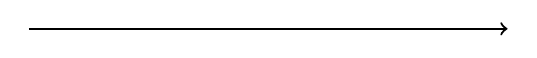
\begin{tikzpicture}[scale=0.8]
  % TODO: pre-drawn display
  \draw[->, thick] (-0.2,0) -- (7.4,0);
\end{tikzpicture}
\end{center}
\\
& TODO: one sentence that reads the display, with a \blank{1.3cm} fill.
\notesprompt{TODO Read the display.}
\begin{probgrid}{|Y|Y|Y|}
\pcell{7}{TODO}{0.9cm}{} & \pcell{8}{TODO}{0.9cm}{} & \pcell{9}{TODO}{0.9cm}{} \\ \hline
\pcell{10}{TODO}{1.3cm}{} & \pcell{11}{TODO}{1.3cm}{} & \pcell{12}{TODO}{1.3cm}{} \\ \hline
\end{probgrid}
\\ \hline
% ── ROW 3: TODO procedure ────────────────────────────────────────────────────
\mainidea{TODO Label} &
TODO: the setup sentence.

\vspace{3pt}
\stepnum{1}\ TODO step with a \blank{2.0cm} fill.\par
\stepnum{2}\ TODO step.\par
\stepnum{3}\ TODO step.

\vspace{4pt}
\textbf{13.} TODO: a table the student fills (never a graph the student draws).
\notesprompt{TODO Use it.}
\begin{probgrid}{|Y|Y|Y|}
\pcell{14}{TODO}{1.5cm}{} & \pcell{15}{TODO}{1.5cm}{} & \pcell{16}{TODO}{1.5cm}{} \\ \hline
\end{probgrid}
\\ \hline
% ── ROW 4: THE CRUX — the target misconception as problems in a grid ─────────
\mainidea[TODO lead]{TODO Label} &
TODO: the contrast, pre-drawn.

\vspace{2pt}
\fcolorbox{navy}{sky}{\parbox{\dimexpr\linewidth-2\fboxsep-2\fboxrule\relax}{\centering
\textbf{TODO the sentence to land, with a \blank{1.4cm} fill.}}}
\notesprompt{TODO Compare.}
\begin{probgrid}{|Y|Y|}
\pcell{17}{TODO}{1.5cm}{} & \pcell{18}{TODO}{1.5cm}{} \\ \hline
\pcell{19}{TODO --- the crux}{1.5cm}{} & \pcell{20}{TODO --- the counterweight}{1.5cm}{} \\ \hline
\end{probgrid}
\\ \hline
% ── LAST ROW: GUIDED PRACTICE — we do, together, a fresh context ─────────────
\mainidea[Guided practice]{TODO Title} &
TODO: the fresh context in one sentence, then its pre-drawn display.
\\
& \notesprompt{We work these together.}
\begin{probgrid}{|Y|Y|Y|}
\pcell{21}{TODO}{1.4cm}{} & \pcell{22}{TODO}{1.4cm}{} & \pcell{23}{TODO}{1.4cm}{} \\ \hline
\pcell{24}{TODO}{1.6cm}{} & \pcell{25}{TODO --- the crux transferred}{1.6cm}{} & \pcell{26}{TODO}{1.6cm}{} \\ \hline
\end{probgrid}
\\ \hline
\end{guidednotes}

% ── THE NOTES END AT GUIDED PRACTICE ─────────────────────────────────────────
% There is deliberately no "you do" here: ../homework/ is the individual practice,
% started in class in the last 8 minutes while the teacher circulates.

\end{document}
